\documentclass[10pt]{beamer}

\usetheme{metropolis}
\usepackage{appendixnumberbeamer}

\usepackage{booktabs}
\usepackage[scale=2]{ccicons}

\usepackage{pgfplots}
\usepgfplotslibrary{dateplot}

\usepackage{xspace}

\usepackage{tikz}
    \usetikzlibrary{positioning}

%\usepackage{listings}
\usepackage{minted}

\usepackage{bm}%................................. Bold math symbols (after fonts)

\setbeamercolor{normal text}{bg=white}





\title{EML4930/EML6934: Lecture 05}
\subtitle{More NumPy and some matplotlib}
\date{September 28, 2017}
%\author{CJ}
\author{Charles Jekel}
%\titlegraphic{\includegraphics{images/avatarCropped.png}\vspace{58cm}}
%\institute{1. University of Florida\\ 2. Stellenbosch University, South Africa}

% \titlegraphic{\hfill\includegraphics[height=1.5cm]{logo.pdf}}

\begin{document}

\maketitle

\begin{frame}{Reminder Quiz at the end of this class}

\end{frame}

\begin{frame}{Issues with HW?}

\end{frame}

\begin{frame}{What am I going to cover this lecture}
\begin{itemize}
\item review arrays
\item difference between array dimensions
\item array shaping
\item saving and loading numpy arrays
\item matplotlib 
\end{itemize}
\end{frame}

\begin{frame}[fragile]{Let's consider these two arrays}
\begin{minted}
{python}
import numpy as np
a = np.array([6, 9, 2, 3, 6])
b = np.array([[6], [9], [2], [3], [6]])

# what are the dimensions
print(a.ndim)
print(b.ndim)

# what are the shapes
print(a.shape)
print(b.shape)

# let's print the transpose of a
print(a)
print(a.T)

\end{minted}
\end{frame}

\begin{frame}[fragile]{Let's consider these two arrays}
\begin{minted}
{python}
# let's print the transpose of b
c = b.T
print(b)
print(c)

# what has change?
print(b.shape)
print(c.shape)

# what is the difference between the following?
print(a*a)
print(np.dot(a,a))
\end{minted}
\end{frame}

\begin{frame}[fragile]{Saving NumPy arrays}
\mint{python}|np.save(file, arr)|
Save an array to a binary file in NumPy .npy format.
\mint{python}|np.save('a_vect',a)|
This creates a\_vect.npy file of the vector a.
\end{frame}

\begin{frame}[fragile]{Loading NumPy arrays}
\mint{python}|np.load(file)|
Load arrays or pickled objects from .npy, .npz or pickled files.
\mint{python}|a_vect = np.load('a_vect.npy')|
This loads the a\_vect.npy binary file into the a\_vect vector.
\end{frame}

\begin{frame}[fragile]{Saving NumPy arrays as plain text and loading the file}
\mint{python}|np.savetxt(fname,X)|
Save the array X to a text file fname.
\mint{python}|a = numpy.loadtxt(fname)|
Load data from a text file named fname and store this as array a.

Each row in the text file must have the same number of values.
\end{frame}

\begin{frame}[fragile]{NumPy reshape}
\begin{minted}
{python}
a = np.arange(6)
b = a.reshape((3,2))
c = a.reshape((2,3))
d = a.reshape((6,1))
print(b)
print(c)
print(d)

out:
[[0 1]
 [2 3]
 [4 5]]
[[0 1 2]
 [3 4 5]]
[[0 1 2 3 4 5]]
\end{minted}
\end{frame}

\begin{frame}[fragile]{NumPy array concatenation - or joining}
\begin{minted}
{python}
x = np.array([4, 5, 0, 3, 7])
y = np.array([3, 4, 9, 7, 5])
z = np.concatenate([x,y])
print(z)

# you can you use np.vstack to vertically stack arrays
w = np.vstack([x,y])

# you can use np.hstack to horizontally stack arrays
v = np.hstack([w,w])
\end{minted}
\end{frame}

\begin{frame}[fragile]{flatten any ndarray into one dimension}
\begin{minted}
{python}
k = np.random.random((5,3,2,6,8))
print(k.ndim)
k_flat = k.flatten()
print(k_flat.ndim)
print(k_flat.size)

out:
5
1
1440
\end{minted}
\end{frame}

\begin{frame}{matplotlib}
Matplotlib tries to make easy things easy and hard things possible. You can generate plots, histograms, power spectra, bar charts, errorcharts, scatterplots, etc., with just a few lines of code. For a sampling, see the screenshots, thumbnail gallery, and examples directory

For simple plotting the pyplot module provides a MATLAB-like interface, particularly when combined with IPython. For the power user, you have full control of line styles, font properties, axes properties, etc, via an object oriented interface or via a set of functions familiar to MATLAB users.

\url{https://matplotlib.org/}
\end{frame}

\begin{frame}{For reference}
Dr. Jake VanderPlas’s Python Data Science Handbook: Essential Tools for Working with Data.

Chapter 4: Visualization with Matplotlib

\url{http://nbviewer.jupyter.org/github/jakevdp/PythonDataScienceHandbook/blob/master/notebooks/Index.ipynb}
\end{frame}

\begin{frame}[fragile]{matplotlib pyplot - MATLAB like plotting framework}
\begin{minted}
{python}
import numpy as np
import matplotlib.pyplot as plt

x = np.linspace(0.0, 2.0*np.pi, 25)

# you can specify a figure number or string name
# but by default plt.figure() will create a number ordered 
# figure name Ex: plt.figure('my figure') or plt.figure(1)
plt.figure() 
# create a line plot by default
plt.plot(x,np.cos(x))
# show the plot
plt.show()
\end{minted}
\end{frame}

\begin{frame}{matplotlib linestyles}
\begin{table}
\begin{tabular}{ll}
\textbf{Linestyle} & \textbf{Description}  \\
\hline
'-' or 'solid' 	 &  solid line\\
'--' or 'dashed' &	dashed line\\
'-.' or 'dashdot'& 	dash-dotted line\\
':' or 'dotted'  &	dotted line\\
'None'           &	draw nothing\\
' '              &	draw nothing\\
'' 	             &  draw nothing\\
\end{tabular}
\end{table}
\end{frame}

\begin{frame}[fragile]{Plotting cosine with a dashed line}
\begin{minted}
{python}
import numpy as np
import matplotlib.pyplot as plt

x = np.linspace(0.0, 2.0*np.pi, 25)

plt.figure() 

# all you need to do is pass the linestyle as an attribute
plt.plot(x,np.cos(x), '--')
plt.show()
\end{minted}
\end{frame}

\begin{frame}{Scatter plot markers}
and more at - \url{https://matplotlib.org/api/markers_api.html} 
\begin{table}
\begin{tabular}{ll}
\textbf{Marker} & \textbf{Description}  \\
\hline
"." &	point\\
"," &	pixel\\
"o" &	circle\\
"v" &	triangle\_down\\
"$<$" &	triangle\_left\\
"$>$" &	triangle\_right\\
"1" &	tri\_down\\
"2" &	tri\_up\\
"3" &	tri\_left\\
"4" &	tri\_right\\
"8" &	octagon\\
"s" &	square\\
"p" &	pentagon\\
"P" &	plus (filled)\\
\end{tabular}
\end{table}
\end{frame}

\begin{frame}[fragile]{Scatter plot cosine}
\begin{minted}
{python}
import numpy as np
import matplotlib.pyplot as plt

x = np.linspace(0.0, 2.0*np.pi, 25)

plt.figure() 

# all you need to do is pass the marker into plot
plt.plot(x,np.cos(x), 'o')
plt.show()
\end{minted}
\end{frame}

\begin{frame}[fragile]{You can easily combine markers and linestyles}
\begin{minted}
{python}
import numpy as np
import matplotlib.pyplot as plt

x = np.linspace(0.0, 2.0*np.pi, 25)

plt.figure() 

# this will plot a -- linestyle with circles at the data points
plt.plot(x,np.cos(x), '--o')
plt.show()
\end{minted}
\end{frame}

\begin{frame}{basic built-in colors in matplotlib}
and more at - \url{https://matplotlib.org/api/colors_api.html} 
\begin{table}
\begin{tabular}{ll}
\textbf{Code} & \textbf{Color}  \\
\hline
b & blue\\
g & green\\
r & red\\
c & cyan\\
m & magenta\\
y & yellow\\
k & black\\
w & white\\
\end{tabular}
\end{table}
\end{frame}

\begin{frame}[fragile]{You can specify the built in color into plot}
\begin{minted}
{python}
import numpy as np
import matplotlib.pyplot as plt

x = np.linspace(0.0, 2.0*np.pi, 25)

plt.figure() 

# forcing the line and dot color to be blue
plt.plot(x,np.cos(x), 'b--o')
plt.show()
\end{minted}
\end{frame}

\begin{frame}[fragile]{Alternatively use color=''}
\begin{minted}
{python}
# specify color by name 
plt.plot(x, np.cos(x), color='blue')

# short color code (rgbcmyk)
plt.plot(x, np.cos(x), color='g') 

# Grayscale between 0 and 1                   
plt.plot(x, np.cos(x), color='0.75')        

# Hex code (RRGGBB from 00 to FF) 
plt.plot(x, np.cos(x), color='#FFDD44')     

# RGB tuple, values 0 and 1 
plt.plot(x, np.cos(x), color=(1.0,0.2,0.3)) 

# all HTML color names supported
plt.plot(x, np.cos(x), color='chartreuse') 
\end{minted}
\end{frame}

\begin{frame}[fragile]{Adjusting the plot with axes limit}
\begin{minted}
{python}
import numpy as np
import matplotlib.pyplot as plt

x = np.linspace(0.0, 2.0*np.pi, 25)

plt.figure() 
plt.plot(x,np.cos(x), 'b--o')

# set the x axis limit
plt.xlim(-1,7)

# set the y axis limit
plt.ylim(-2,2)

plt.show()
\end{minted}
\end{frame}

\begin{frame}[fragile]{Adding a grid}
\url{https://matplotlib.org/api/pyplot_api.html?highlight=matplotlib%20pyplot%20grid#matplotlib.pyplot.grid}

grid(b=None, which='major', axis='both', **kwargs)

    kwargs are used to set the grid line properties, e.g.,:
    \mint{python}|ax.grid(color='r', linestyle='-', linewidth=2)|
\begin{minted}
{python}
import numpy as np
import matplotlib.pyplot as plt
x = np.linspace(0.0, 2.0*np.pi, 25)
plt.figure() 
plt.plot(x,np.cos(x), 'b--o')
# create a grid
plt.grid(True)
plt.show()
\end{minted}
\end{frame}

\begin{frame}[fragile]{Labels and legend}
\begin{minted}
{python}
import numpy as np
import matplotlib.pyplot as plt
x = np.linspace(0.0, 2.0*np.pi, 25)
plt.figure() 

# add label='my_label'
plt.plot(x,np.cos(x), '--o', label='cos')
plt.plot(x,np.sin(x), '-.s', label='sin')
plt.grid(True)

# add legend
plt.legend()
# legend automatically chooses the location
# but you can specify the simple quadrant based location as
# plt.legend(loc=1) puts the legend in the first quadrant

plt.show()
\end{minted}
\end{frame}

\begin{frame}[fragile]{matplotlib title and axis label}
\begin{minted}
{python}
import numpy as np
import matplotlib.pyplot as plt
x = np.linspace(0.0, 2.0*np.pi, 25)
plt.figure() 
plt.plot(x,np.cos(x), '--o', label='cos')
plt.plot(x,np.sin(x), '-.s', label='sin')
plt.grid(True)
plt.legend()
# adding a title
plt.title('Cos and sin')

# x and y axis labels
plt.xlabel('x axis')
plt.ylabel('y axis')

plt.show()
\end{minted}
\end{frame}

\begin{frame}[fragile]{matplotlib pyplot savefig}
\url{https://matplotlib.org/api/pyplot_api.html?highlight=matplotlib%20pyplot%20savefig#matplotlib.pyplot.savefig}

\begin{minted}
{python}
plt.savefig(fname, dpi=None, facecolor='w', edgecolor='w',
        orientation='portrait', papertype=None, format=None,
        transparent=False, bbox_inches=None, pad_inches=0.1,
        frameon=None)
\end{minted}

How I normally create publication quality pictures:
\begin{minted}
{python}
plt.savefig('my_fig.pdf', dpi=600, format='pdf',
            bbox_inches='tight')
\end{minted}
 Most backends support png, pdf, ps, eps and svg.
\end{frame}

\begin{frame}[fragile]{saving my cosine and sin plot}
Depending on your active Python interpreter, you'll have issues with plt.show()
\begin{minted}
{python}
import numpy as np
import matplotlib.pyplot as plt
x = np.linspace(0.0, 2.0*np.pi, 25)
plt.figure() 
plt.plot(x,np.cos(x), '--o', label='cos')
plt.plot(x,np.sin(x), '-.s', label='sin')
plt.grid(True)
plt.legend()
plt.xlabel('x axis')
plt.ylabel('y axis')

plt.savefig('my_fig.pdf', dpi=600, format='pdf',
             bbox_inches='tight')
\end{minted}
\end{frame}

\begin{frame}{Created this plot}
\begin{figure}
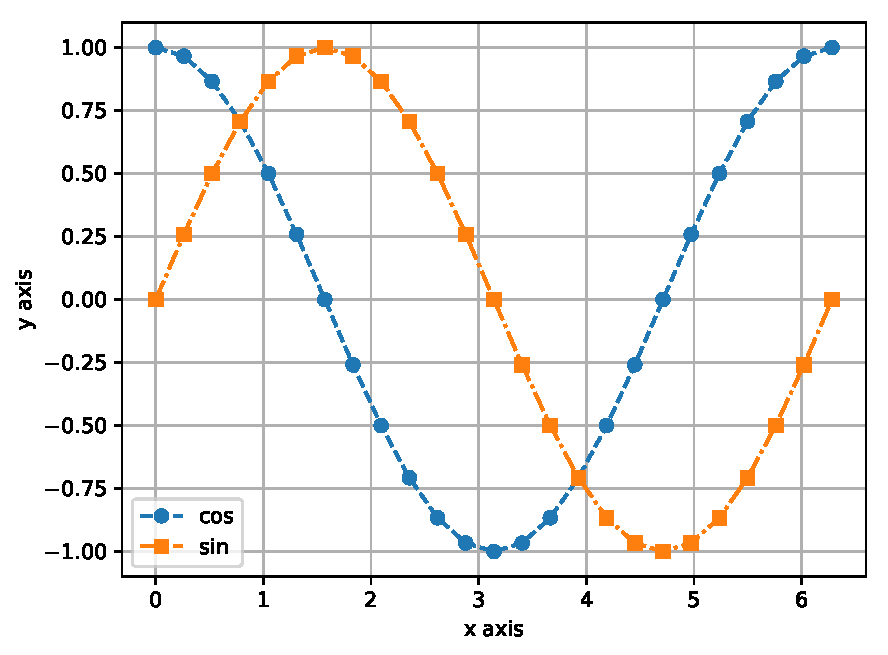
\includegraphics[width=0.9\textwidth]{fig/my_fig.pdf}
\end{figure}
\end{frame}


%\begin{frame}{Quiz at the end of next class}
%There will be a quiz at the end of next class. 
%
%The quiz will be 3 short questions. 
%
%10 sample quiz questions are posted online. You should know how to answer each one of these questions. The 3 questions asked will be very similar to these 10 questions.
%\end{frame}
%
%\begin{frame}{Concerns about HW?}
%
%\end{frame}
%
%\begin{frame}{Reference for this lecture}
%This lecture will cover chapter 2 of Python Data Science Handbook by VanderPlas. 
%
%\url{http://nbviewer.jupyter.org/github/jakevdp/PythonDataScienceHandbook/blob/master/notebooks/Index.ipynb}
%\end{frame}
%
%\begin{frame}{NumPy - \url{http://numpy.org}}
%NumPy is the fundamental package for scientific computing with Python. It contains among other things:
%\begin{itemize}
%\item a powerful N-dimensional array object
%\item sophisticated (broadcasting) functions
%\item tools for integrating C/C++ and Fortran code
%\item useful linear algebra, Fourier transform, and random number capabilities
%\item documentation \url{https://docs.scipy.org/doc/numpy-1.13.0/reference/index.html}
%\end{itemize}
%\end{frame}
%
%\begin{frame}{If you're coming from MATLAB read}
%\url{https://docs.scipy.org/doc/numpy-dev/user/numpy-for-matlab-users.html}
%\end{frame}
%
%\begin{frame}[fragile]{Importing NumPy}
%\begin{minted}
%{python}
%import numpy as np
%\end{minted}
%
%This is the most standard form of how to import the numpy library.
%\end{frame}
%
%
%\begin{frame}[fragile]{What is a NumPy array?}
%	\begin{alertblock}{NumPy ndarray()}
%A n-dimensional arrays of homogeneous data types. 
%	\end{alertblock}
%
%\begin{itemize}
%\item The \textit{ndarray} object is the core of NumPy.
%\item \textit{ndarray} has become the standard Python vector/matrix/tensor types.
%\item Elements of \textit{ndarray} must have the same data type.
%\item Mathematical operations on \textit{ndarray} are more efficient than built-in Python functions.
%\item Much of the code was created in compiled code for performance. 
%\item Documentation \url{https://docs.scipy.org/doc/numpy-1.10.0/reference/arrays.ndarray.html}
%\end{itemize}
%\end{frame}
%
%\begin{frame}[fragile]{NumPy array attributes - memory layout}
%The following attributes contain information about the memory layout of the array:
%\begin{itemize}
%\item ndarray.flags - Information about the memory layout of the array.
%\item ndarray.shape -	Tuple of array dimensions.
%\item ndarray.strides -	Tuple of bytes to step in each dimension when traversing an array.
%\item ndarray.ndim -	Number of array dimensions.
%\item ndarray.data -	Python buffer object pointing to the start of the array’s data.
%\item ndarray.size -	Number of elements in the array.
%\item ndarray.itemsize - 	Length of one array element in bytes.
%\item ndarray.nbytes - 	Total bytes consumed by the elements of the array.
%\item ndarray.base -	Base object if memory is from some other object.
%\end{itemize}
%\end{frame}
%
%\begin{frame}[fragile]{NumPy array attributes - other attributes}
%The following attributes contain information about the memory layout of the array:
%\begin{itemize}
%\item ndarray.dtype -	Data-type of the array’s elements.
%\item ndarray.T -	Same as self.transpose(), except that self is returned if self.ndim $<$ 2.
%\item ndarray.real - 	The real part of the array.
%\item ndarray.imag -	The imaginary part of the array.
%\item ndarray.flat -	A 1-D iterator over the array.
%\item ndarray.ctypes -	An object to simplify the interaction of the array with the ctypes module.
%\end{itemize}
%\end{frame}
%
%\begin{frame}{NumPy array methods - array conversion 1 of 2}
%\begin{itemize}
%\item ndarray.item(*args) - 	Copy an element of an array to a standard Python scalar and return it.
%\item ndarray.tolist() -	Return the array as a (possibly nested) list.
%\item ndarray.itemset(*args) -	Insert scalar into an array (scalar is cast to array's dtype, if possible) There must be at least 1 argument, and define the last argument as item.
%\item ndarray.tostring([order]) -	Construct Python bytes containing the raw data bytes in the array.
%\item ndarray.tobytes([order]) - 	Construct Python bytes containing the raw data bytes in the array.
%\item ndarray.tofile(fid[, sep, format]) -	Write array to a file as text or binary (default).
%\item ndarray.dump(file) -	Dump a pickle of the array to the specified file.
%\item ndarray.dumps() -	Returns the pickle of the array as a string.
%\item ndarray.astype(dtype[, order, casting, ...]) -	Copy of the array, cast to a specified type.
%\end{itemize}
%\end{frame}
%
%\begin{frame}{NumPy array methods - array conversion 2 of 2}
%\begin{itemize}
%\item ndarray.byteswap(inplace) -	Swap the bytes of the array elements Toggle between low-endian and big-endian data representation by returning a byteswapped array, optionally swapped in-place.
%\item ndarray.copy([order]) -	Return a copy of the array.
%\item ndarray.view([dtype, type]) -	New view of array with the same data.
%\item ndarray.getfield(dtype[, offset]) -	Returns a field of the given array as a certain type.
%\item ndarray.setflags([write, align, uic]) -	Set array flags WRITEABLE, ALIGNED, and UPDATEIFCOPY, respectively.
%\item ndarray.fill(value) -	Fill the array with a scalar value.
%\end{itemize}
%\end{frame}
%
%\begin{frame}{NumPy array methods - shape manipulation}
%\begin{itemize}
%\item ndarray.reshape(shape[, order]) -	Returns an array containing the same data with a new shape.
%\item ndarray.resize(new\_shape[, refcheck]) - 	Change shape and size of array in-place.
%\item ndarray.transpose(*axes) -	Returns a view of the array with axes transposed.
%\item ndarray.swapaxes(axis1, axis2) -	Return a view of the array with axis1 and axis2 interchanged.
%\item ndarray.flatten([order]) -	Return a copy of the array collapsed into one dimension.
%\item ndarray.ravel([order]) -	Return a flattened array.
%\item ndarray.squeeze([axis]) -	Remove single-dimensional entries from the shape of a.
%\end{itemize}
%\end{frame}
%
%\begin{frame}{Numpy array methods - methods that are also functions}
%\begin{columns}
%\begin{column}{0.3\textwidth}
%\begin{itemize}
%\item all
%\item any
%\item argmax
%\item argmin
%\item argpartition
%\item argsort
%\item choose
%\item clip
%\item compress
%\item copy
%\item cumprod
%\item cumsum
%\item diagonal
%\end{itemize}
%
%\end{column}
%\begin{column}{0.3\textwidth} 
%\begin{itemize}
%\item imag
%\item max
%\item mean
%\item min
%\item nonzero
%\item partition
%\item prod
%\item ptp 
%\item put
%\item ravel
%\item real
%\item repeat
%\end{itemize}
%\end{column}
%\begin{column}{0.3\textwidth} 
%\begin{itemize}
%\item reshape
%\item round
%\item searchsorted
%\item sort
%\item squeeze
%\item std
%\item sum
%\item swapaxes
%\item take
%\item trace
%\item transpose
%\item var
%\end{itemize}
%\end{column}
%\end{columns}
%\end{frame}
%
%\begin{frame}{NumPy array data types - 1 of 2}
%\begin{table}
%\begin{tabular}{ll}
%\textbf{Type} & \textbf{Description}  \\
%\hline
%bool\_ 	  &  Boolean (True or False) stored as a byte \\
%int\_ 	    &  Default integer type (normally either int64 or int32) \\
%intc 	    &  Identical to C int (normally int32 or int64) \\
%intp 	    &  Integer used for indexing (normally either int32 or int64) \\
%int8 	    &  Byte (-128 to 127) \\
%int16 	  &  Integer (-32768 to 32767) \\
%int32 	  &  Integer (-2147483648 to 2147483647) \\
%int64 	  &  Integer (-9223372036854775808 to 9223372036854775807) \\
%uint8 	  &  Unsigned integer (0 to 255) \\
%uint16 	  &  Unsigned integer (0 to 65535) \\
%uint32 	  &  Unsigned integer (0 to 4294967295) \\
%uint64 	  &  Unsigned integer (0 to 18446744073709551615) \\
%\end{tabular}
%\end{table}
%\end{frame}
%\begin{frame}{NumPy array data types - 2 of 2}
%NumPy arrays support a larger variety of data types than the default Python!
%\begin{table}
%\begin{tabular}{ll}
%\textbf{Type} & \textbf{Description}  \\
%\hline
%float\_ 	  &  Shorthand for float64. \\
%float16 	&  Half precision: sign bit, 5 bits exponent, 10 bits mantissa \\
%float32 	&  Single precision: sign bit, 8 bits exponent, 23 bits mantissa \\
%float64 	&  Double precision: sign bit, 11 bits exponent, 52 bits mantissa \\
%complex\_ 	&  Shorthand for complex128. \\
%complex64 &	Complex number, represented by two 32-bit floats  \\
%complex128 & 	Complex number, represented by two 64-bit floats  \\
%\end{tabular}
%\end{table}
%\end{frame}
%
%\begin{frame}[fragile]{NumPy array creation - from lists}
%Use \mint{python}|np.array(list)|
%to create an array from a Python list
%
%Examples:
%\begin{minted}
%{python}
%# one dimensional array shape (4,)
%x = np.array([1, 2, 4, 6])
%
%# two dimensional array shape (2,2)
%y = np.array([[1 ,2], [2, 3]])
%
%# three dimensional array - shape (2,2,2)
%z = np.array([[[1 ,2], [2, 3]], [[1 ,2], [2, 3]]])
%\end{minted}
%\end{frame}
%
%\begin{frame}[fragile]{NumPy array creation - specify data type}
%You can specify the data type of the array using \mint{python}|np.array(list, dtype=)|
%
%Examples:
%\begin{minted}
%{python}
%# one dimensional array - Byte
%x = np.array([1, 2, 4, 6], dtype='int8')
%
%# two dimensional array - Single precision
%y = np.array([1, 2, 4, 6], dtype='float32')
%
%# three dimensional array - Double precision
%z = np.array([1, 2, 4, 6], dtype='float64')
%\end{minted}
%
%\end{frame}
%
%\begin{frame}[fragile]{NumPy array creation - display data type}
%You can view the data type with \mint{python}|ndarray.dtype)|
%
%Examples:
%\begin{minted}
%{python}
%in : x.dtype
%out: dtype('int8')
%
%in : y.dtype
%out: dtype('float32')
%
%in : z.dytpe
%out: dtype('float64')
%\end{minted}
%\end{frame}
%
%\begin{frame}[fragile]{Default data types follow python convention}
%
%If you include a decimal point NumPy array will default to double precision floating point.
%
%Examples:
%\begin{minted}
%{python}
%in : a = np.array(1); a.dtype
%out: dtype('int32')
%
%in : b = np.array(1.); b.dtype
%out: dtype('float64')
%
%in : c = np.array([1,1.]); c.dtype
%out: dtype('float64')
%
%in : d = np.array([1., 1, 1, 1, 1, 1, 1]); d.dtype
%out: dtype('float64')
%\end{minted}
%\end{frame}
%
%\begin{frame}[fragile]{NumPy array creation - from scratch 1 of 3}
%These default to double precision floating point unless otherwise specified.
%\begin{minted}
%{python}
%# Create a length-10 integer array filled with zeros
%np.zeros(10, dtype=int)
%
%# Create a 3x5 floating-point array filled with 1s
%np.ones((3, 5), dtype=float)
%
%# Create a 3x5 array filled with 3.14
%np.full((3, 5), 3.14)
%
%# Create an array filled with a linear sequence
%# Starting at 0, ending at 20, stepping by 2        
%np.arange(0, 20, 2)
%\end{minted}
%\end{frame}
%
%\begin{frame}[fragile]{NumPy array creation - from scratch 2 of 3}
%\begin{minted}
%{python}
%# Create an array of five values evenly spaced between 0 and 1
%np.linspace(0, 1, 5)
%
%# Create a 3x3 array of uniformly distributed
%# random values between 0 and 1
%np.random.random((3, 3))
%
%# Create a 3x3 array of normally distributed random values
%# with mean 0 and standard deviation 1
%np.random.normal(0, 1, (3, 3))
%
%# Create a 3x3 array of random integers in the interval [0, 10)
%np.random.randint(0, 10, (3, 3))
%
%# Create a 3x3 identity matrix
%np.eye(3)
%\end{minted}
%\end{frame}
%
%\begin{frame}[fragile]{NumPy array creation - from scratch 3 of 3}
%\begin{minted}
%{python}
%# Create an uninitialized array of three integers
%# The values will be whatever happens to already exist at that
%# memory location        
%np.empty(3)
%\end{minted}
%\end{frame}
%
%\begin{frame}[fragile]{Seeding NumPy pseudorandom number generator}
%Use seed to ensure that the arrays are the same for each time the code is run.
%
%\begin{minted}
%{python}
%# seed for reproducibility
%np.random.seed(0)  
%
%# One-dimensional array 
%x1 = np.random.randint(10, size=6)
%
%# Two-dimensional array        
%x2 = np.random.randint(10, size=(3, 4))
%
%# Three-dimensional array          
%x3 = np.random.randint(10, size=(3, 4, 5))  
%\end{minted}
%\end{frame}
%
%\begin{frame}[fragile]{NumPy array - useful attributes}
%\begin{minted}
%{python}
%# the number of dimensions
%print("x3 ndim: ", x3.ndim)
%
%# the size of each dimension of the array 
%print("x3 shape:", x3.shape)
%
%# the total size of the array   
%print("x3 size: ", x3.size)
%
%# the item size (in bytes) of each array element       
%print("itemsize:", x3.itemsize, "bytes")
%
%# the total size (in bytes) of the array   
%print("itemsize:", x3.nbytes, "bytes")
%\end{minted}
%\end{frame}
%
%\begin{frame}[fragile]{NumPy array indexing - one dimensional}
%One dimensional arrays index just like lists
%\begin{minted}
%{python}
%x = np.array([2, 3, 4, 9])
%
%# print the first item
%print(x[0])
%
%# print the second item
%print(x[1])
%
%# print the last item
%print(x[-1])
%\end{minted}
%\end{frame}
%
%\begin{frame}[fragile]{NumPy array indexing - two dimensional}
%Two dimensional arrays also index just like lists! 
%\begin{minted}
%{python}
%y = np.array([[1,2], [3,4]])
%
%# print 1 from y
%print(y[0,0])
%
%# print 2 from y
%print(y[0,1])
%
%# print 3 from y
%print(y[1,0])
%
%# print 4 from y
%print(y[1,1])
%\end{minted}
%\end{frame}
%
%\begin{frame}[fragile]{NumPy array slicing - just like list slicing!}
%\begin{minted}
%{python}
%in : x = np.array([0, 1, 2, 3, 4, 5, 6, 7, 8, 9])
%in : x[:5]  # first five elements
%out: array([0, 1, 2, 3, 4])
%
%in : x[5:]  # elements after index 5
%out: array([5, 6, 7, 8, 9])
%
%in : x[4:7]  # middle subarray
%out: array([4, 5, 6])
%
%in : x[::2]  # every other element
%out: array([0, 2, 4, 6, 8])
%
%in : x[1::2]  # every other element, starting at index 1
%out: array([1, 3, 5, 7, 9]) 
%
%in : x[::-1]  # all elements, reversed
%out: array([9, 8, 7, 6, 5, 4, 3, 2, 1, 0])
%\end{minted}
%\end{frame}
%
%\begin{frame}[fragile]{NumPy array - rows and columns of}
%\begin{minted}
%{python}
%in : x = np.array([[12,  5,  2,  4],
%                   [ 7,  6,  8,  8],
%                   [ 1,  6,  7,  7]])
%
%# first column of x
%x[:,0]
%
%# second column of x
%x[:,1]
%
%# third row of x
%x[2,:]
%
%# first row of x
%x[0,:]
%\end{minted}
%\end{frame}
%
%\begin{frame}[fragile]{NumPy array - assigning individual values}
%\begin{minted}
%{python}
%in : x = np.array([[12,  5,  2,  4],
%                   [ 7,  6,  8,  8],
%                   [ 1,  6,  7,  7]])
%
%x[0,0] = 0
%x[0,1] = 1
%x[0,2] = 2
%x[0,3] = 3
%print(x)
%
%out: array([[ 0,  1,  2,  3],
%            [ 7,  6,  8,  8],
%            [ 1,  6,  7,  7]])
%\end{minted}
%\end{frame}
%
%\begin{frame}[fragile]{NumPy arrays pass by reference!}
%use copy() if you want a copy of the data!
%
%\begin{minted}
%{python}
%a = np.ones(3)
%b = a
%c = a.copy()
%
%a *= 7
%print('a:', a)
%print('b:', b)
%print('c:', c)
%\end{minted}
%\end{frame}
%
%\begin{frame}{NumPy aggregration functions}
%\begin{table}
%\begin{tabular}{lll}
%\textbf{Function} & \textbf{NaN-safe} & \textbf{Description}  \\
%\hline
%np.sum          & np.nansum        & Compute sum of elements\\
%np.prod         & np.nanprod       & Compute product of elements\\
%np.mean         & np.nanmean       & Compute median of elements \\
%np.std          & np.nanstd        & Compute standard deviation \\
%np.var          & np.nanvar        & Compute variance \\
%np.min          & np.nanmin        & Find minimum value \\
%np.max          & np.nanmax        & Find maximum value \\
%np.argmin       & np.nanargmin     & Find index of minimum value \\
%np.argmax       & np.nanargmax     & Find index of maximum value \\
%np.median       & np.nanmedian     & Compute median of elements \\
%np.percentile   & np.nanpercentile & Compute rank-based statistics of elements \\
%np.any          & N/A Evaluate     & whether any elements are true \\
%np.all          & N/A Evaluate     & whether all elements are true\\
%\end{tabular}
%\end{table}
%\end{frame}
%
%\begin{frame}[fragile]{NumPy useful functions}
%\begin{minted}
%{python}
%np.abs(x) # absolute value
%
%# trig functions
%np.sin(x)
%np.cos(x)
%np.tan(x)
%np.arcsin(x)
%np.arccos(x)
%np.arctan(x)
%
%
%np.exp(x)  # e^x
%np.log(x)  # natural log
%np.log2(x) # log base 2
%np.log10(x)# log base 10
%\end{minted}
%\end{frame}
%
%\begin{frame}[fragile]{NumPy arrays - arithmetic operators}
%\begin{table}
%\begin{tabular}{ll}
%\textbf{Operator} & \textbf{Description}  \\
%\hline
% + & Addition (e.g., 1 + 1 = 2)\\
% - & Subtraction (e.g., 3 - 2 = 1) \\
% - & Unary negation (e.g., -2) \\
% * & Multiplication (e.g., 2 * 3 = 6) \\
%/  & Division (e.g., 3 / 2 = 1.5) \\
%// & Floor division (e.g., 3 // 2 = 1) \\
%** & Exponentiation (e.g., 2 \*\* 3 = 8) \\
% \% & Modulus/remainder (e.g., 9 \% 4 = 1)\\
%\end{tabular}
%\end{table}
%\end{frame}
%
%\begin{frame}[fragile]{NumPy arrays - element wise math}
%\begin{minted}
%{python}
%in :
%a = np.array([2, 4, 6, 8])
%b = np.array([3, 4, 5, 6])
%
%print(a+b)
%print(a-b)
%print(a*b)
%print(a**b)
%
%out: 
%[ 5  8 11 14]
%[-1  0  1  2]
%[ 6 16 30 48]
%[     8    256   7776 262144]
%\end{minted}
%\end{frame}
%
%\begin{frame}[fragile]{NumPy arrays - element wise math}
%\begin{minted}
%{python}
%in :
%a = np.array([[2, 4],[6, 8]])
%b = np.array([[3, 4],[5, 6]])
%print(a+b)
%print(a-b)
%print(a*b)
%print(a**b)
%
%out: 
%[[ 5  8]
% [11 14]]
%[[-1  0]
% [ 1  2]]
%[[ 6 16]
% [30 48]]
%[[     8    256]
% [  7776 262144]]
%\end{minted}
%\end{frame}
%
%\begin{frame}[fragile]{NumPy arrays - dot product}
%Use np.dot(a,b) to take the dot product of arrays a and b
%
%\begin{minted}
%{python}
%in :
%a = np.array([2, 4, 6, 8])
%b = np.array([3, 4, 5, 6])
%print(np.dot(a,b))
%
%out: 100
%\end{minted}
%\end{frame}
%
%\begin{frame}[fragile]{NumPy arrays - dot product for matrix multiplication}
%The dot product of two dimensional arrays is matrix multiplication
%
%\begin{minted}
%{python}
%in :
%x = np.array([[4, 5, 2],
%              [7, 7, 1],
%              [9, 1, 7]])
%y = np.eye(3)
%
%print(np.dot(x,y))
%
%out: 
%[[4, 5, 2],
% [7, 7, 1],
% [9, 1, 7]])
%\end{minted}
%\end{frame}
%
%\begin{frame}[fragile]{NumPy linear algebra - decomposition}
%\begin{table}
%\begin{tabular}{ll}
%\textbf{function} & \textbf{Description}  \\
%\hline
%np.linalg.cholesky(a) & Cholesky decomposition \\
%np.linalg.qr(a[,mode]) & qr factorization \\
%np.linalg.svd(a[, full\_matrices, compute\_uv]) & Singular value decomposition \\
%\end{tabular}
%\end{table}
%\end{frame}
%
%\begin{frame}[fragile]{NumPy linear algebra - eigenvalues}
%\begin{minted}
%{python}
%in :
%w, v = np.linalg.eig(np.diag((1, 2, 3)))
%
%print(w)
%print(v)
%
%out: 
%array([ 1.,  2.,  3.])
%array([[ 1.,  0.,  0.],
%       [ 0.,  1.,  0.],
%       [ 0.,  0.,  1.]])
%\end{minted}
%\end{frame}
%
%\begin{frame}{NumPy linear algebra - norms and other numbers}
%\begin{table}
%\begin{tabular}{ll}
%\textbf{Function} & \textbf{Description}  \\
%\hline
%np.linalg.norm(x) 	     & Matrix or vector norm.\\
%np.linalg.cond(x) 	     & Compute the condition number of a matrix.\\
%np.linalg.det(a) 	       & Compute the determinant of an array.\\
%np.linalg.matrix\_rank(M) & Return matrix rank of array using SVD method.\\
%np.linalg.slogdet(a) 	   & Sign and $\ln$ of the determinant of an array.\\
%np.trace(a) 	           & Return the sum along diagonals of the array.\\
%\end{tabular}
%\end{table}
%\end{frame}
%
%\begin{frame}{NumPy linear algebra - solving equations and inverting matrices}
%\begin{table}
%\begin{tabular}{ll}
%\textbf{Function} & \textbf{Description}  \\
%\hline
%np.linalg.solve(a, b) 	            &  Solve a linear matrix equation\\
%np.linalg.tensorsolve(a, b[, axes]) &	Solve the tensor equation a x = b for x\\
%np.linalg.lstsq(a, b[, rcond]) 	    &  least-squares solution to a linear equation\\
%np.linalg.inv(a) 	                  & multiplicative) inverse of a matrix\\
%np.linalg.pinv(a[, rcond])    	    &  (Moore-Penrose) pseudo-inverse of a matrix\\
%np.linalg.tensorinv(a[, ind]) 	    &  ‘inverse’ of an N-dimensional array\\
%\end{tabular}
%\end{table}
%\end{frame}
%
%\begin{frame}[fragile]{Don't invert arrays! Use solve!}
%np.linalg.solve automatically uses parallel processing if it suspects using multiple threads will be faster!
%\begin{minted}
%{python}
%F = np.array([[2.0, 3.0],
%              [-2.0,9.0]])
%c = np.array([ 12.9,  12.3])
%
%# solve the equation Fa = c for a
%a = np.linalg.solve(F,c)
%
%# check the solution
%print(np.dot(F,a))
%\end{minted}
%\end{frame}



\end{document}
